\chapter{Foundations}

This chapter presents the theory and models applied in this thesis. First, the details of the communication problem is described, then the mathematical theory of the frameworks used to model this problem is introduced.

\section{Problem Formulation}
\begin{wrapfigure}{r}{4cm}
	\begin{center}
		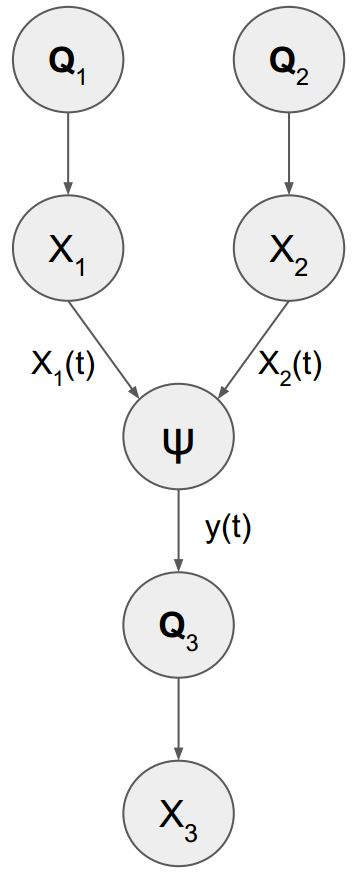
\includegraphics[width=2.5cm]{figures/h_model}
		\caption{Graphical model.}
	\end{center}
	\label{wrap-fig:1}
\end{wrapfigure} 
The communication model considered in this thesis is given in Figure \ref{wrap-fig:1}. The parent nodes, $X_{1}$ and $ X_{2}$, emit messages which carry information about their states. These messages are translated by an observation model, $\psi$, and agent node, $ X_{3} $ makes a decision based on this translated message, $ y $. The main objective is to infer the observation model given the trajectories of nodes.

The messages that are emitted by the parent nodes $X_{1}$ and $ X_{2} $ are modelled as independent homogeneous continuous-time Markov processes $X_{i}(t)$, with state space $ \rchi_{i} = \left\lbrace x_{1}, x_{2}, ..., x_{n} \right\rbrace  $ for $ i \in \left\lbrace 1,2 \right\rbrace $. These processes are defined by transition intensity matrices $ Q_{i} $, where intensities do not depend on time. These matrices are assumed to be gamma distributed.
\begin{equation}
\textbf{Q}_{i} \sim Gam(\alpha_{i}, \beta_{i})\ \ for\ i \in \left\lbrace 1,2\right\rbrace \nonumber
\end{equation}
The agent node does not have a direct access to the messages, but observes a translation of them. The observation model is defined as the likelihood of a translation given the parent messages.
\begin{equation}
\psi \coloneqq p(y(t) \mid X_{1}(t), X_{2}(t))
\end{equation}
The agent  $ X_{3} $ is modelled as inhomogeneous continuous-time Markov process with state space $ \rchi_{3} = \left\lbrace x_{1}, x_{2}, ..., x_{n} \right\rbrace  $, set of actions $ a \in \left\lbrace a_{0}, a_{1}, ..., a_{k}\right\rbrace  $ and set of transition intensity matrices $ \textbf{\textit{Q}}_{3} = \left\lbrace \textbf{Q}_{a_{0}}, \textbf{Q}_{a_{1}}, ..., \textbf{Q}_{a_{k}} \right\rbrace $. 
\begin{equation}
\textbf{Q}_{a} \sim Gam(\alpha_{a}, \beta_{a})
\end{equation}
Given the observation, the agent forms a belief over the parent states, $  b(x_{1}, x_{2}; t) $, that summarizes the past observations.\cite{Kaelbling2011} The policy of the agent, $ \pi(a \mid b) $, is assumed to be shaped by evolution (close) to optimality. Based on the belief state, the agent takes an action, which in the setting described above means to change its internal dynamics through choice of intensity matrix. 

\section{Continuous Time Markov Processes}

A continuous-time Markov process (CTMP) is a continuous-time stochastic process which satisfies Markov property, namely, the probability distribution over the states at a future time is conditionally independent of the past states given the current state.\cite{Cohn2010a} Let X be a CTMP with state space $ \rchi = \left\lbrace x_{1}, x_{2}, ..., x_{n} \right\rbrace  $. Then the Markov property can be written as follows:
\begin{equation}
	\operatorname{Pr}\left(X^{\left(t_{k}\right)}=x_{t_{k}} | X^{\left(t_{k-1}\right)}=x_{t_{k-1}}, \ldots, X^{\left(t_{0}\right)}=x_{t_{0}}\right)=\operatorname{Pr}\left(X^{\left(t_{k}\right)}=x_{t_{k}} | X^{\left(t_{k-1}\right)}=x_{t_{k-1}}\right)
\end{equation}
A CTMP is represented by its transition intensity matrix, $ \textbf{Q} $. In this matrix, the intensity $ q_{i} $ represents the instantaneous probability of leaving state $ x_{i} $ and $ q_{i,j} $ represents the instantaneous probability of switching from state $ x_{i} $ to $ x_{j} $. 
\begin{equation}
	\textbf{Q} = 
	\begin{bmatrix}
	-q_{1} & q_{1,2} & 	{\hdots}  & q_{1,n} \\
	q_{2,1} & -q_{2} & 	{\hdots}  & q_{2,n}  \\
	{\vdots}  & 	{\vdots}  & 	{\ddots}  & {\hdots}  \\
	q_{n,1} &  q_{n,2} &  {\hdots} & -q_{n}
	\end{bmatrix}
\end{equation}
where $ q_{i} = \sum_{i \neq j} q_{i,j}$.\cite{Nodelman1995}

\subsection{Homogenous Continuous Time Markov Processes}
A continuous-time Markov process is time-homogenous when the transition intensities do not depend on time. Let X be a homogenous CTMP, with transition intensity matrix \textbf{Q}. Infinitesimal transition probability from state $ x_{i} $ to $ x_{j} $ in terms of the transition intensities $ q_{i,j} $ can be written as \cite{Cohn2010a}:
\begin{equation}
p_{i,j}(h)=\delta_{ij}+q_{i,j} h+o(h)
\end{equation}
where $ p_{i, j}(h) \equiv Pr(X^{(t+h)}=j\mid X^{(t)}=i) $ are Markov transition functions and o(.) is a function decaying to zero faster than its argument.

The \textit{master equation} is then derived as follows:
\begin{align}
	p_{j}(t) &= \operatorname{Pr}(X(t) = x_{j}) \nonumber\\
		& =\sum_{\forall i} p_{i, j}(h) p_{i}(t-h) \nonumber \\
	\lim_{h\rightarrow 0} p_{j}(t) 
		& = \lim_{h\rightarrow 0} \sum_{\forall i} \left[ \delta_{ij}+q_{i,j} h+o(h)\right]  p_{i}(t-h) \nonumber \\ 
		& = \lim_{h\rightarrow 0} p_{j}(t-h) + \lim_{h\rightarrow 0} h \sum_{\forall i} q_{i,j} p_{i}(t-h) \nonumber \\
	\lim_{h\rightarrow 0} \frac{p_{j}(t) - p_{j}(t-h)}{h} 
		&= \lim_{h\rightarrow 0} \sum_{\forall i} q_{i,j} p_{i}(t-h) \nonumber\\
	\frac{d}{dt} p_{j}(t) & = \sum_{\forall i} q_{i,j} p_{i}(t)
%		& = \sum_{\forall i \neq j}\left[  q_{i,j} p_{i}(t) - q_{j,i} p_{j}(t) \right]\nonumber
	\label{eq:master_equation}
\end{align}
Eq.\ref{eq:master_equation} can be written in matrix form:
\begin{equation}
\frac{d}{dt} p(t) = p(t)\textbf{Q}
\end{equation}
where the time-dependent probability distribution $ p(t) $ is a row vector with entries $ {p_{i}(t)}_{x_{i}\in \rchi} $. 
The solution of this ODE is, 
\begin{equation}
p(t)=p(0) \exp (t\textbf{Q})
\end{equation}
with initial distribution $ p(0) $.

The amount of time staying in a state $ x_{i} $ is exponentially distributed with parameter $ q_{i} $. The probability density function $ f $ and cumulative distribution function $ F $ for staying in the state $ x_{i} $ \cite{Nodelman1995}:
\begin{align}
f(t) & = q_{i} \exp \left(-q_{i} t\right), t\geq 0  \label{eq:f(t)_homo}\\
F(t) & = 1 - \exp \left(-q_{i} t\right), t\geq 0 
\end{align}
Given the transitioning from state $ x_{i} $, the probability of landing on state $ x_{j} $ is $ q_{i,j}/q_{i} $.
\subsubsection{Likelihood Function}
Consider a single transition denoted as $ d = <x_{i},x_{j},t> $, where transition occurs from state $ x_{i} $ to $ x_{j} $ after spending t amount of time at state $ x_{i} $. The likelihood of this transition is the product of the probability of having remained at state $ x_{i} $ for that long, and the probability of transitioning to $ x_{j} $.
\begin{equation}
\operatorname{Pr}(d  \mid \textbf{Q}) = \left( q_{i}exp(-q_{i}t) \right) \left( \frac{q_{i,j}}{q_{i}} \right)
\end{equation}
The likelihood of a trajectory sampled from a homogenous CTMC, $ X^{[0,T]} $, can be decomposed as the product of the likelihood of single transitions. The sufficient statistics summarizing this trajectory can be written as $ T[x_{i}] $, total amount of time spent in state $ x_{i} $, $ M[x_{i}, x_{j}] $ total number of transitions from state $ x_{i} $ to $ x_{j} $, we can write down the likelihood of a trajectory $  X^{\left[0,T\right] } $,
\begin{align}
\operatorname{Pr}(X^{[0,T]}  \mid \textbf{Q}) &=  \prod_{d \in X^{[0,T]}} \operatorname{Pr}(d \mid \textbf{Q}) \nonumber\\&=\left(\prod_{ i} q_{i}^{M[x_{i}]} \exp \left(-q_{i} T[x_{i}]\right)\right)\left(\prod_{ i} \prod_{ j \neq i} \left(\frac{q_{i,j}}{q_{i}}\right)^{M\left[x_{i}, x_{j}\right]}\right) \nonumber\\ & = \prod_{i}  exp(-q_{i}T[x_{i}]) \prod_{j \neq i}  q_{i,j}^{M[x_{i},x_{j}]}
\label{eq:lh_traj_homo}
\end{align}
where $ M[x_{i}] = \sum_{j \neq i} M[x_{i}, x_{j}] $ is the total number transitions leaving state $ x_{i} $.

\subsubsection{Marginalized Likelihood Function} 
Let $ X $ be a homogenous CTMP. For convenience, it is assumed to be binary-valued, $ \rchi = \left\lbrace x_{0}, x_{1} \right\rbrace $. The transition intensity matrix can be written in the following form:
\begin{equation}
\textbf{Q} = 
\begin{bmatrix}
-q_{0} & q_{0} \\
q_{1} & -q_{1}
\end{bmatrix}
\end{equation}
where the transition intensities $ q_{0} $ and $ q_{1} $ are gamma-distributed with parameters $ \alpha_{0}$, $ \beta_{0} $ and $ \alpha_{1} $, $ \beta_{1} $, respectively. The marginal likelihood of a sample trajectory $ X^{[0,T]} $ can be written as follows:
\begin{align}
P(X^{[0, T]}) & = \int  P(X^{[0, T]}\mid Q)P(Q) dQ \nonumber\\ & = \int_{0}^{\infty} \left( \prod_{x} \exp(-q_{x}T_{x}) \prod_{x'} q_{xx'}^{M[x, x']}\right) \frac{\beta_{xx'}^{\alpha_{xx'}}{q_{xx'}^{\alpha_{xx'}-1}}\exp(-\beta_{xx'}q_{xx'})}{\Gamma(\alpha_{xx'})} \ dq_{xx'} \nonumber\\ & = \prod_{i\in{0,1}}\int_{0}^{\infty} q_{i}^{M[x_{i}]} \ \exp(-q_{i}T[x_{i}]) \  \frac{\beta_{i}^{\alpha_{i}} \ q_{i}^{\alpha_{i}-1}\ \exp(-\beta_{i}q_{i})}{\Gamma(\alpha_{i})} \ dq_{i} \nonumber\\ & = \prod_{i\in{0,1}} \frac{\beta_{i}^{\alpha_{i}}}{\Gamma(\alpha_{i})} \int_{0}^{\infty} q_{i}^{M[x_{i}] + \alpha_{i} -1} \ \exp(-q_{i}(T[x_{i}]+\beta_{i})) \ dq_{i} \\ & = \prod_{i\in{0,1}} \frac{\beta_{i}^{\alpha_{i}}}{\Gamma(\alpha_{i})} \left( -(T_{i}+\beta_{i})^{M[x_{i}] + \alpha_{i}}\ \Gamma(M[x_{i}] + \alpha_{i}, \ q_{i}(T[x_{i}]+\beta_{i})) \right) \Big|_0^\infty  \\ & = \prod_{i\in{0,1}} \frac{\beta_{i}^{\alpha_{i}}}{\Gamma(\alpha_{i})} \left( (T[x_{i}]+\beta_{i})^{M[x_{i}] + \alpha_{i}}\ \Gamma(M[x_{i}] + \alpha_{i}) \right)
\label{eq:Marg_traj}
\end{align}.
%
%where $ T[x_{i}] $, the amount of time spent in state $ [x_{i}] $, $ M[x_{i},x_{j}] $ the number of transitions from state $ x_{i} $ to $ x_{j} $ and  $ M[x_{i}] = \sum_{i\neq j}M[x_{i},x_{j}] $.\\

%From Eq.11, the integral is solved using computer algebra system WolframAlpha as follows:
%\begin{align}
%\int x^{a} \ \exp(-xb) \ dx = -b^{-a-1} \ \Gamma(a+1, \ bx) + C
%\label{eq:integral}
%\end{align}
%
%Plugging Eq.\ref{eq:Marg_traj} in Eq.\ref{eq:Marg_llh} for both $ X_{1} $ and $ X_{2} $:
%\begin{align}
%\begin{split}
%P(\textit{D} \mid \pi, \Phi ) = P(X_{3}^{[0, T]}\mid Q_{3}^{[0, T]}) \prod_{x_{1}\in{0,1}} \frac{\beta_{x_{1}}^{\alpha_{x_{1}}}}{\Gamma(\alpha_{x_{1}})} \ (T_{x_{1}}+\beta_{x_{1}})^{M_{x_{1}} + \alpha_{x_{1}}}\ \Gamma(M_{x_{1}} + \alpha_{x_{1}})  \\  \prod_{x_{2}\in{0,1}} \frac{\beta_{x_{2}}^{\alpha_{x_{2}}}}{\Gamma(\alpha_{x_{2}})} \ (T_{x_{2}}+\beta_{x_{2}})^{M_{x_{2}} + \alpha_{x_{2}}}\ \Gamma(M_{x_{2}} + \alpha_{x_{2}})
%\label{eq:Marg_llh_final}
%\end{split}
%\end{align}
\subsection{Inhomogeneous Continuous Time Markov Processes}
%In an conventional CTBN, while every node is a Markov process itself, the leaf nodes are \textit{conditional} Markov processes, a type of inhomogeneous Markov process, where the intensities change over time, but not as a function of time rather as a function of parent states. \cite{Nodelman1995} %TODO explain time-dependence in the problem
A continuous-time Markov process is time-inhomogenous when the transition intensities changes over time.
For CTMP, Eq.\ref{eq:f(t)_homo} becomes:
\begin{equation}
f(t) = q_{i}(t) \exp \left(-\int_{0}^{t} q_{i}(u) d u\right)
\end{equation}
\subsubsection{Likelihood Function}
Let X be an inhomogeneous Markov process. $  X^{\left[0,T\right] } $ is a trajectory sampled from this process with $ m $ number of transitions, $ 0 = t_{0} < t_{1} < ... < t_{m} $ are the times where transition occurred, and $ x_{t_{0}}, x_{t_{1}},..., x_{t_{m}} $ are the observed states. The likelihood of trajectory  $  X^{\left[0,T\right] } $ can be written as follows: 
\begin{equation}
L(\textbf{Q}_{X} \colon  X^{\left[0,T\right]} ) = \prod_{k=1}^{m} \left[ q_{x_{k-1}} (t_{k}) \exp \left(-\int_{t_{k-1}}^{t_{k}} q_{x_{k-1}}(u) d u\right) \frac{q_{x_{k-1}, x_{k}} (t_{k})}{q_{x_{k-1}}(t_{k})}\right] 
\label{eq:lh_traj_inhomo}
\end{equation}

%We can formulate our graphical model as $ S = [X, Y, Z] $, where $ Par(Z) = {X,Y} $ and $ Par(X) = Par(Y) =\emptyset $. We can then write the conditional probability:
%\begin{equation}
%\begin{split}
%P\left(S^{\left(t+h\right)}=s' | S^{\left(t\right)}=s\right) = & P\left(X^{\left( t+h\right) }=x' | X^{\left(t\right)}=x, Par(X)^{\left(t\right)}={y,z}\right) \\&  P\left(Y^{\left( t+h\right) }=y' | Y^{\left(t\right)}=y\right) P\left(Z^{\left( t+h\right) }=z' | ^{\left(t\right)}=z\right)
%\end{split} 
%\end{equation}

\section{Belief State in Partially Observable Markov Decision Processes}
Partially observable Markov decision process (POMDP) framework provides a model of an agent which interacts with its environment, but unable to obtain certain information about its state. Instead, the agent gets an observation which is a stochastic function of the true state. The main goal, as similar to Markov decision processes (MDPs), is to learn a policy solving a task by optimizing a reward function. The problem of decision making under uncertainty can be decomposed into two parts for the agent. The first is to keep a belief state which is a sufficient statistic of its past experiences, and the second is to generate an optimal policy which will give an action based on the belief state. \cite{Murphy2000,Kaelbling2011}

In the problem considered in this thesis, the agent node $ X_{3} $ cannot observe the incoming messages directly, rather a summary of them. This presents a POMDP problem. However, since the optimal policy of the agent is assumed to be given, the theory for policy optimization is skipped. In this section, update methods for belief state is introduced.

In the following, belief state refers to the posterior probability distribution over the environment states.

\subsection{Exact/Bayes(?) Belief State Update}

Consider a POMDP problem, with state space \textit{S}, action space \textit{A}, observation space $ \Omega $. In a scneario where a compact representation of the \textit{transition model}, $ T(s, a, s^{\prime})$,  and \textit{observation model}, $ O(s^{\prime}, a, o) $, is available, the belief state update can be obtain via Bayes' theorem \cite{Kaelbling2011}:
\begin{align}
b^{\prime}\left(s^{\prime}\right) &=\operatorname{Pr}\left(s^{\prime} | o, a, b\right) \nonumber\\
&=\frac{\operatorname{Pr}\left(o | s^{\prime}, a, b\right) \operatorname{Pr}\left(s^{\prime} | a, b\right)}{\operatorname{Pr}(o | a, b)} \nonumber\\
&=\frac{\operatorname{Pr}\left(o | s^{\prime}, a\right) \sum_{s \in \mathcal{S}} \operatorname{Pr}\left(s^{\prime} | a, b, s\right) \operatorname{Pr}(s | a, b)}{\operatorname{Pr}(o | a, b)} \nonumber\\
&=\frac{O\left(s^{\prime}, a, o\right) \sum_{s \in \mathcal{S}} T\left(s,a, s^{\prime}\right) b(s)}{\operatorname{Pr}(o | a, b)}
\label{eq:discrete_belief_update}
\end{align}

\subsection{Filtering for CTMP}
Eq.\ref{eq:discrete_belief_update} is discrete-time solution of belief state. However, since in the model described in Section 2.1, the parent nodes are modelled as CTMPs, and the environment state for the agent is the state of an CTMP, the belief state should be solved in continuous-time. This is achieved by the inference of posterior probability of CTMP.
%To derive \textit{continuous-time belief state}, $ b(t) $, first we need to get the joint transition matrix of X and Y, two independent processes. This operation called \textit{amalgamation} is described in detail by Nodelman \textit{et al} \cite{Nodelman1995}. 
%Let us denote this matrix by $ Q_{XY} $. 

Let X be a CTMC with transition intensity matrix \textbf{Q}. Assume discrete-time observations denoted by $ y_{1}=y(t_{1}), ..., y_{N}=y(t_{N}) $. The belief state can be written as:
\begin{equation}
	b(x_{i};t_{N}) = \operatorname{Pr}(X(t_{N}) = x_{i} \mid y_{1}, ..., y_{N})
\end{equation}
From the master equation given in Eq.\ref{eq:master_equation}, it follows that:
\begin{equation}
 \frac{d}{dt} b(x_{j};t)  = \sum_{\forall i} q_{i,j} b(x_{i};t)
\end{equation}
The time-dependent belief state $ b(t) $ is a row vector with $ \left\lbrace b(x_{i};t)_{x_{i} \in \rchi}\right\rbrace  $.
This posterior probability can be described by a system of ODEs:
\begin{equation}
\frac{db(t)}{dt} = b(t)\textbf{Q}
\end{equation}
where the initial condition $ b(0) $ is row vector with $ \left\lbrace b(x_{i};t)_{x_{i} \in \rchi}\right\rbrace $ \cite{article}.

The belief state update at discrete times of observation $ y_{t} $ is derived as 
\begin{align}
b(x_{i}; t_{N}) & = \operatorname{Pr}( X(t_{N}) = x_{i},\mid y_{1}, ..., y_{N}) \nonumber\\ & = \frac{\operatorname{Pr}(y_{1}, ..., y_{N}, X(t_{N}) = x_{i})}{\operatorname{Pr}(y_{1}, ..., y_{N})}  \nonumber\\ & = \frac{\operatorname{Pr}(y_{N} \mid y_{1}, ..., y_{N-1}, X(t_{N}) = x_{i})}{\operatorname{Pr}(y_{N} \mid y_{1}, ..., y_{N-1})} \frac{\operatorname{Pr}(y_{1}, ..., y_{N-1}, X(t_{N}) = x_{i})}{\operatorname{Pr}(y_{1}, ..., y_{N-1})}  \nonumber\\ & = Z_{N}^{-1} \ \operatorname{Pr}(y_{N} \mid X(t_{N})=x_{i})\ \operatorname{Pr}( X(t_{N}) = x_{i}\mid y_{1}, ..., y_{N-1})  \nonumber\\ & = Z_{N}^{-1}\ {\operatorname{Pr}(y_{N} \mid X(t_{N})=x_{i})}\ {b(x_{i}; t_{N}^{-})}
\end{align}
where $ Z_{N} = \sum_{x_{i}\in \rchi} \operatorname{Pr}(y_{N} \mid X(t_{N})=x_{i})\ b(x_{i}; t_{N}^{-}) $ is the normalization factor \cite{article}.

\subsection{Belief State Update using Particle Filter}
In a more realistic scenario, the exact update of belief state may not be feasible for several reasons. 
%TODO explain why do we need particle filter, how is this in the literature, how did we end up here


\subsubsection{Marginalized Continuous Time Bayesian Networks}
%The marginal process description of a CTMC/CTBN is given as 
%\begin{multline}
%p(X_n(t + dt) = x' \mid X_n(t)=x, U_n(t)=u, X_{[0, t)})\\
%\begin{split}
%&= \int p(X_n(t + dt) = x' \mid X_n(t)=x, U_n(t)=u, Q^u_n, X_{[0, t)})p(Q^u_n)dQ^u_n\\
%&= \delta(x, x') + \underbrace{\mathbb{E}[Q^u_n (x, x') \mid X_{[0, t]} = x_{[0, t]}]}_{\equiv f^u_n(x'\mid x_{[0, t]})}dt + o(dt),
%\end{split}
%\end{multline}
%where we introduced $f$ for brevity. This expression also holds for $K$ trajectories that have been independently drawn from the CTBN; in line with the paper, we denote the joint history of all $K$ trajectories until time point $t$ as $\xi_t = \{x^1_{[0, t]}, ..., x^K_{[0, t]}\}$.
%
%\bigskip
%By integrating out the rate matrices $Q^u_n$, we introduced dependencies between all trajectories; this is readily seen by evaluation of the above expectation:
%\begin{align}
%\mathbb{E}[Q^u_n (x, x') \mid \xi_t] &=\frac{\alpha^u_n(x, x') + r^u_n(x, x')}{\beta^u_n(x, x') + T^u_n(x)}\\
%&=\frac{\alpha^u_n(x, x') + \sum_k r^u_{n, k}(x, x')}{\beta^u_n(x, x') + \sum_k T^u_{n, k}(x)}.
%\end{align}
%The expectation of the rate matrix depends on the summary statistics $T^u_n = \sum_k T^u_{n,k}$, $r^u_n = \sum_k r^u_{n,k}$ from all observed trajectories up to the current point in time. Hence, to draw $K$ trajectories from a marginalised CTBN exactly, they have to be simulated jointly, inducing a joint path measure $p(\{X^k_{[0, T]} : k = 1, ..., K\})$.
%Because this is computationally infeasible, we would like to approximate this resulting joint distribution
%by a set of $K$ factorising variational distributions: $\prod_k q(X^k_{[0, T]})$ such that
%\begin{equation}
%\min_q \mathrm{KL}\,\left(\prod_k q(X^k_{[0, T]})\mid\mid p(\{X^k_{[0, T]}\}_k)\right).
%\end{equation}


\subsubsection{Particle Filter}
%TODO The explaination and the algorithm

\scalebox{1}{\begin{algorithm}[H]
		\KwIn{Measurement data $ y_{k} $ at time $ t_{k} $, set of particles $\textbf{p}^{k-1} $, estimated $ \hat{Q} $}
		\KwResult{New set of particles $ \textbf{p}^{k} $, representing $ b(t_{k}) $}
		\vspace{+4pt}
		\begin{algorithmic}[1]
			\FOR{$p_{m} \in \textbf{p}^{k-1}$}
			\STATE {$p_{m} = \left\lbrace x_{m}, \hat{Q}\right\rbrace \leftarrow Propagate\ particle\ through\ marginal\ process\ model\ from\ t_{k-1}\ to\ t_{k}$ }
			\STATE{$w_{m} \leftarrow p(y_{k} \mid X(t_{k})=x_{m}) $} 
			\tcp*[h] {observation likelihood}
			\STATE {$\hat{Q} \leftarrow sufficient\ statistics\ added\ from\  p_{m}[t_{k-1}, t_{k}]$}
			\ENDFOR
			\STATE{$ w_{m} \leftarrow \frac{w_{m}}{\sum_{m} w_{m}}$} \tcp*[h]{normalize weights}
			\FOR{$ p_{m} \in \textbf{p}_{k} $} 
			\STATE{$ p_{m} \leftarrow Sample\ from\ p_{k}\ with\ probabilities\ w_{m}\ with\ replacement$}
			\ENDFOR
		\end{algorithmic}
		\caption{Marginal particle filter}
\end{algorithm}}

\section{Likelihood Model of Communication System (?)}